\documentclass[aspectratio=169]{beamer}
\mode<presentation>
% \usetheme{Warsaw}
% \usetheme{Goettingen}
\usetheme{Hannover}
% \useoutertheme{default}

% \useoutertheme{infolines}
\useoutertheme{sidebar}
\usecolortheme{dolphin}

\usepackage{amsmath}
\usepackage{amssymb}
\usepackage{enumerate}

% some bold math symbosl
\newcommand{\Cov}{\mathrm{Cov}}
\newcommand{\Cor}{\mathrm{Cor}}
\newcommand{\Var}{\mathrm{Var}}
\newcommand{\brho}{\boldsymbol{\rho}}
\newcommand{\bSigma}{\boldsymbol{\Sigma}}
\newcommand{\btheta}{\boldsymbol{\theta}}
\newcommand{\bbeta}{\boldsymbol{\beta}}
\newcommand{\bmu}{\boldsymbol{\mu}}
\newcommand{\bW}{\mathbf{W}}
\newcommand{\one}{\mathbf{1}}
\newcommand{\bH}{\mathbf{H}}
\newcommand{\by}{\mathbf{y}}
\newcommand{\bolde}{\mathbf{e}}
\newcommand{\bx}{\mathbf{x}}

\newcommand{\cpp}[1]{\texttt{#1}}

\title{Mathematical Biostatistics Boot Camp: Lecture 8, Asymptotics}
\author{Brian Caffo}
\date{\today}
\institute[Department of Biostatistics]{
  Department of Biostatistics \\
  Johns Hopkins Bloomberg School of Public Health\\
  Johns Hopkins University
}


\begin{document}

\frame{\titlepage}


\section{Table of contents}
\frame{
  \frametitle{Table of contents}
  \tableofcontents
}

\section{Limits}
\begin{frame}\frametitle{Numerical limits}
  \begin{itemize}
  \item Imagine a sequence
    \begin{itemize}
    \item $a_1 = .9$,
    \item $a_2 = .99$,
    \item $a_3 = .999$, $\hdots$
    \end{itemize}
  \item Clearly this sequence converges to $1$
  \item Definition of a limit: For any fixed distance we can find a
    point in the sequence so that the sequence is closer to the limit
    than that distance from that point on
  \item $|a_n - 1| = 10^{-n}$
  \end{itemize}
\end{frame}

\begin{frame}\frametitle{Limits of random variables}
  \begin{itemize}
  \item The problem is harder for random variables
  \item Consider $\bar X_n$ the sample average of the first $n$ of
    a collection of $iid$ observations
    \begin{itemize}
    \item Example $\bar X_n$ could be the average of the result of
      $n$ coin flips (i.e. the sample proportion of heads)
    \end{itemize}
  \item We say that $\bar X_n$ {\bf converges in probability} to a limit
    if for any fixed distance the {\em probability} of $\bar X_n$ being
    closer (further away) than that distance from the limit converges to
    one (zero)
  \item $P(|\bar X_n - \mbox{limit}| < \epsilon) \rightarrow 1$ 
  \end{itemize}
\end{frame}

\section{LLN}
\begin{frame}\frametitle{The Law of Large Numbers}
  \begin{itemize}
  \item Establishing that a random sequence converges to a limit is hard
  \item Fortunately, we have a theorem that does all the work for us, called
    the {\bf Law of Large Numbers}
  \item The law of large numbers states that if $X_1,\ldots X_n$ are iid
    from a population with mean $\mu$ and variance $\sigma^2$ then $\bar
    X_n$ converges in probability to $\mu$
  \item (There are many variations on the LLN; we are using a particularly
    lazy one)
  \end{itemize}
\end{frame}

\begin{frame}\frametitle{Proof using Chebyshev's inequality}
  \begin{itemize}
  \item Recall Chebyshev's inequality states that the probability that a random variable
    variable is more than $k$ standard deviations from its mean is less than $1/k^2$
  \item Therefore for the sample mean
    $$
    P\left\{|\bar X_n - \mu| \geq k ~\mbox{sd}(\bar X_n)\right\} \leq 1 / k ^ 2
    $$
  \item Pick a distance $\epsilon$ and let $k = \epsilon / \mbox{sd}(\bar X_n)$
    $$
    P(|\bar X_n - \mu| \geq \epsilon) \leq \frac{\mbox{sd}(\bar X_n)^2}{\epsilon^2}
    = \frac{\sigma^2}{n\epsilon^2}
    $$
  \end{itemize}
\end{frame}


\begin{frame}
  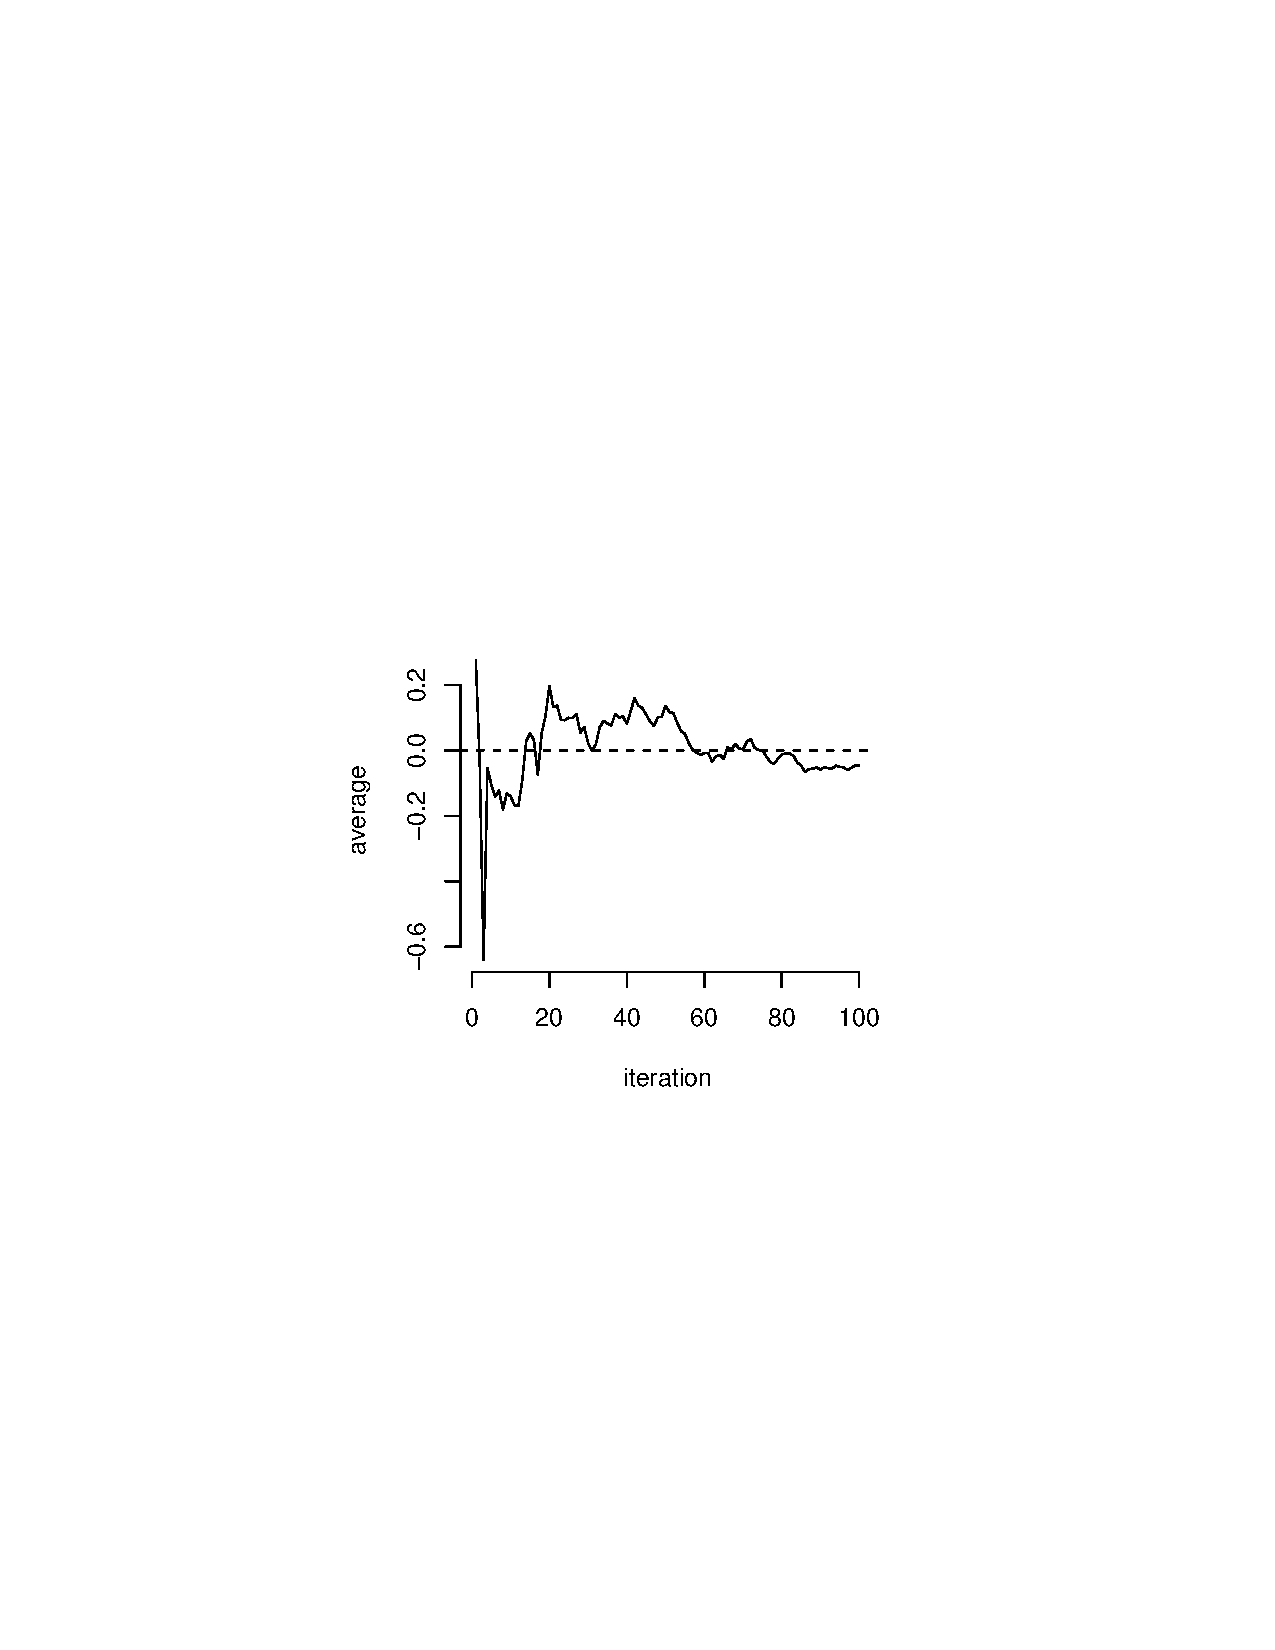
\includegraphics[width=3.5in]{lln.pdf}
\end{frame}

\begin{frame}\frametitle{Useful facts}
  \begin{itemize}
  \item Functions of convergent random sequences converge to 
    the function evaluated at the limit
  \item This includes sums, products, differences, ...
  \item Example $(\bar X_n) ^2$ converges to $\mu^2$
  \item Notice that this is different than $(\sum X_i^2) / n$ which converges
    to $E[X_i^2] = \sigma^2 + \mu^2$
  \item We can use this to prove that the sample variance converges to
    $\sigma^2$
  \end{itemize}
\end{frame}

\begin{frame}\frametitle{Continued}
  \begin{eqnarray*}
    \sum (X_i - \bar X_n)^2 / (n - 1) & =  & \frac{\sum X_i^2}{n - 1}  - \frac{n (\bar X_n)^2}{n - 1}  \\ \\
    & = & \frac{n}{n-1}\times \frac{\sum X_i^2}{n} - \frac{n}{n-1} \times (\bar X_n)^ 2\\ \\
    & \stackrel{p}{\rightarrow} & 1 \times (\sigma^2 + \mu^2) - 1 \times \mu^2 \\ \\
    & = & \sigma^2 
  \end{eqnarray*}
  Hence we also know that the sample standard deviation converges to
  $\sigma$
\end{frame}

\begin{frame}\frametitle{Discussion}
  \begin{itemize}
  \item An estimator is {\bf consistent} if it converges to what you want to estimate
  \item The LLN basically states that the sample mean is consistent
  \item We just showed that the sample variance and the sample standard deviation are
    consistent as well
  \item Recall also that the sample mean and the sample variance are unbiased as well
  \item (The sample standard deviation is biased, by the way)
  \end{itemize}
\end{frame}

\section{CLT}
\begin{frame}\frametitle{The Central Limit Theorem}
  \begin{itemize}
  \item The {\bf Central Limit Theorem} (CLT) is one of the most important theorems in statistics
  \item For our purposes, the CLT states that the distribution of
    averages of iid variables, properly normalized, becomes that of a
    standard normal as the sample size increases
  \item The CLT applies in an endless variety of settings
  \end{itemize}
\end{frame}

\begin{frame}\frametitle{The CLT}
  \begin{itemize}
  \item Let $X_1,\ldots,X_n$ be a collection of iid random variables
    with mean $\mu$ and variance $\sigma^2$
  \item Let $\bar X_n$ be their sample average
  \item Then
    \begin{equation*}
      P\left( \frac{\bar X_n - \mu}{\sigma / \sqrt{n}} \leq z \right) \rightarrow \Phi(z)
    \end{equation*}
  \item Notice the form of the normalized quantity
    $$
    \frac{\bar X_n - \mu}{\sigma / \sqrt{n}} = 
    \frac{\mbox{Estimate} - \mbox{Mean of estimate}}{\mbox{Std. Err. of estimate}}.
    $$
  \end{itemize}
\end{frame}

\begin{frame}\frametitle{Example}
  \begin{itemize}
  \item  Simulate a standard normal random variable by rolling $n$
    (six sided)
  \item Let $X_i$ be the outcome for die $i$
  \item Then note that $\mu = E[X_i] = 3.5$
  \item $\Var(X_i) = 2.92$ 
  \item SE $\sqrt{2.92 / n} = 1.71 / \sqrt{n}$
  \item Standardized mean
    $$
    \frac{\bar X_n - 3.5}{1.71/\sqrt{n}}
    $$ 
  \end{itemize}
\end{frame}

\begin{frame}
  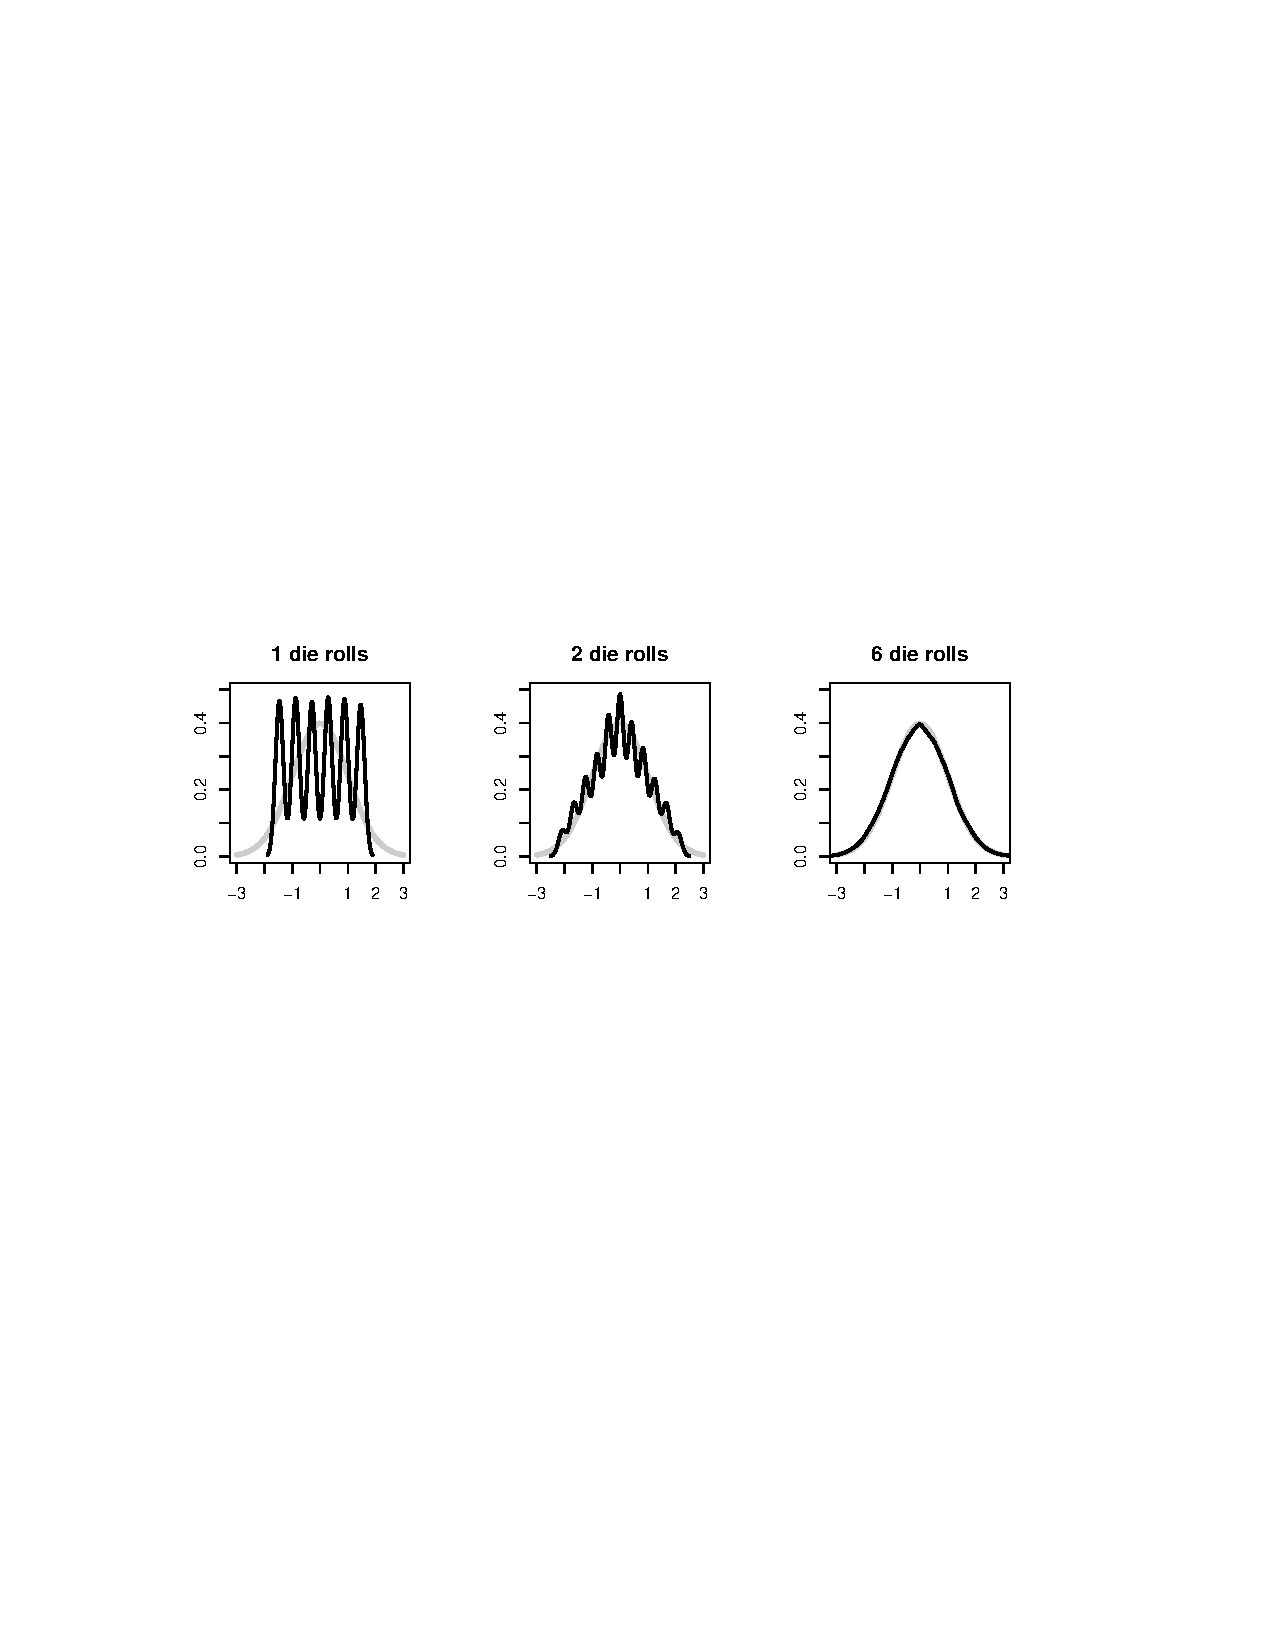
\includegraphics[width=3.5in]{die.pdf}
\end{frame}

\begin{frame}\frametitle{Coin CLT}
  \begin{itemize}
  \item Let $X_i$ be the $0$ or $1$ result of the $i^{th}$ flip of a
    possibly unfair coin
  \item The sample proportion, say $\hat p$, is the average of the coin flips
  \item $E[X_i] = p$ and $\Var(X_i) = p(1-p)$
  \item Standard error of the mean is $\sqrt{p(1-p)/n}$
  \item Then
    $$
    \frac{\hat p - p}{\sqrt{p(1-p)/n}}
    $$
    will be approximately normally distributed
  \end{itemize}
\end{frame}

\begin{frame}
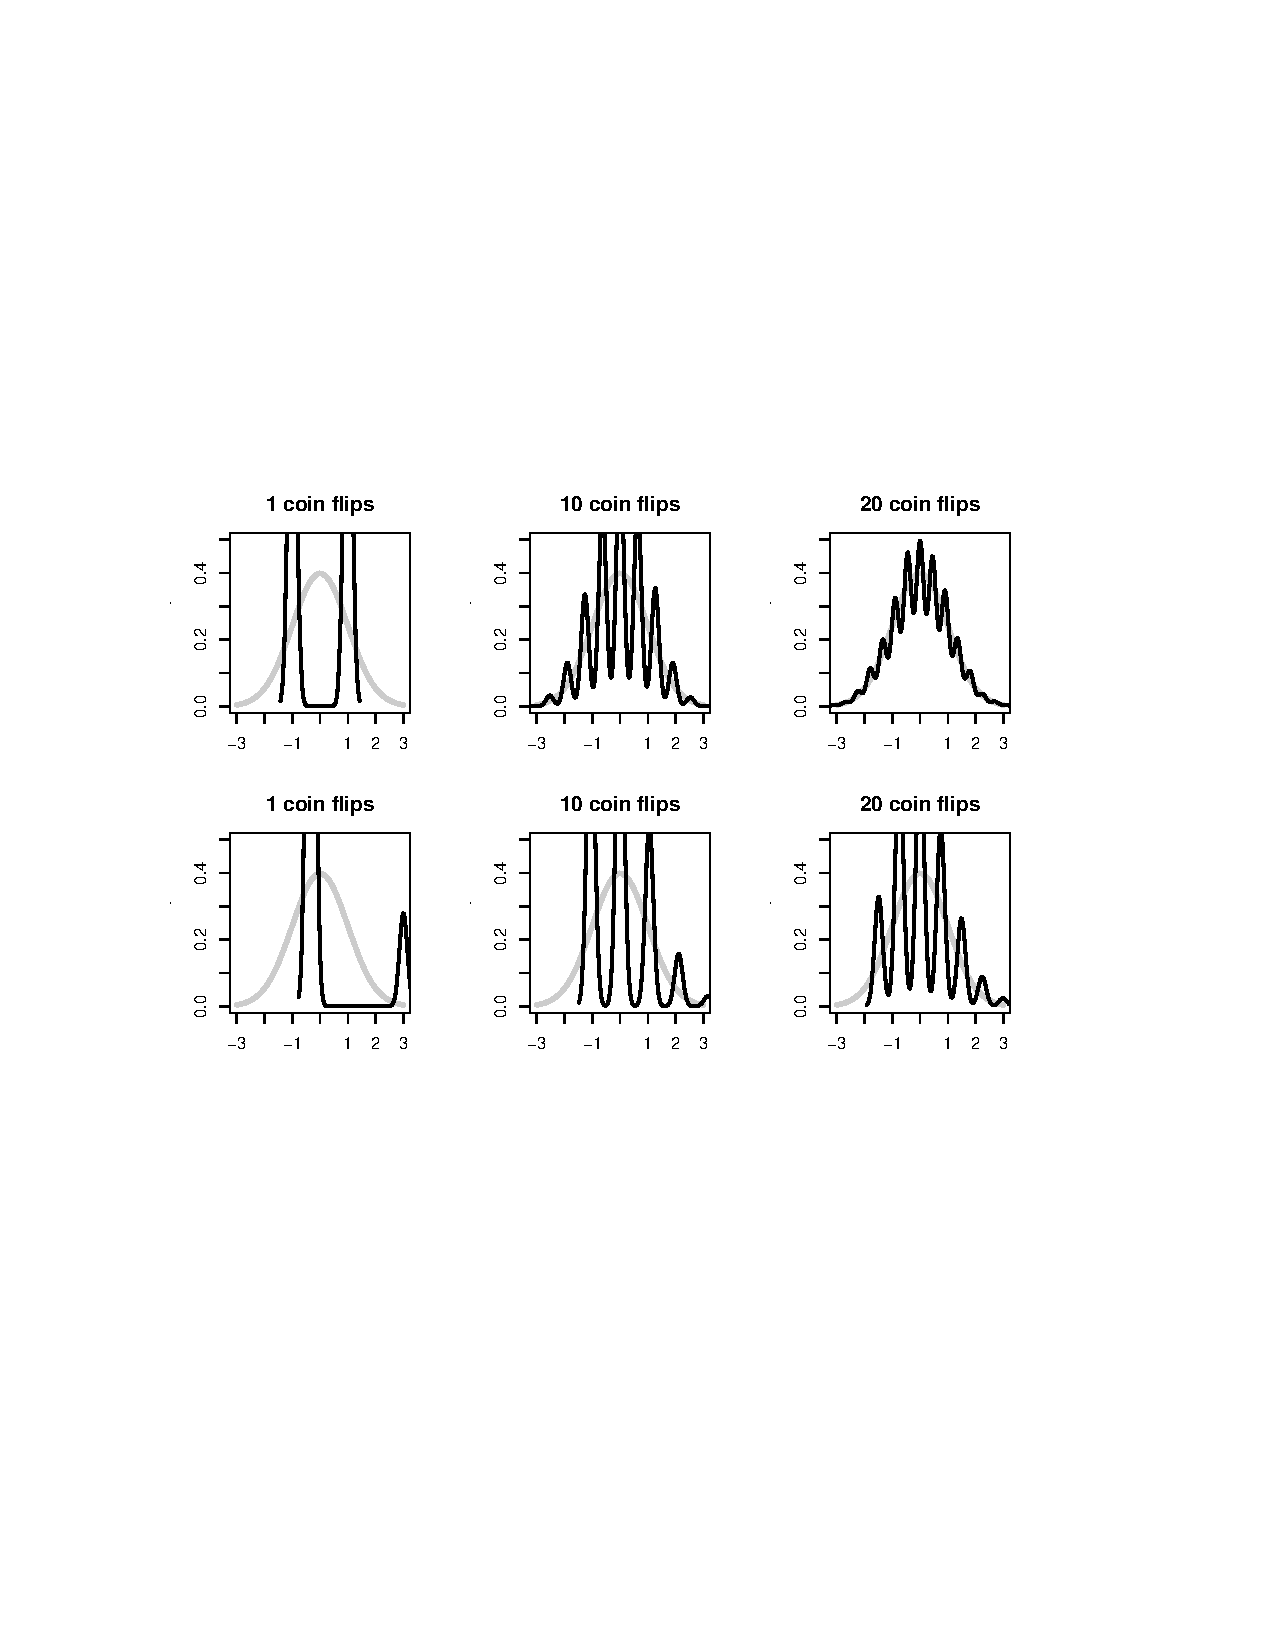
\includegraphics[width=3.5in]{coinCLT.pdf}
\end{frame}

\begin{frame}\frametitle{CLT in practice}
  \begin{itemize}
  \item In practice the CLT is mostly useful as an approximation
    $$
    P\left( \frac{\bar X_n - \mu}{\sigma / \sqrt{n}} \leq z \right) \approx \Phi(z).  
    $$
  \item Recall $1.96$ is a good approximation to the $.975^{th}$
    quantile of the standard normal
  \item Consider
    \begin{eqnarray*}
      .95 & \approx & P\left( -1.96 \leq \frac{\bar X_n - \mu}{\sigma / \sqrt{n}} \leq 1.96 \right)\\ \\
      & =       & P\left(\bar X_n +1.96 \sigma/\sqrt{n} \geq \mu \geq \bar X_n - 1.96\sigma/\sqrt{n} \right),\\
    \end{eqnarray*}
  \end{itemize}
\end{frame}

\section{Confidence intervals}
\begin{frame}\frametitle{Confidence intervals}
  \begin{itemize}
  \item Therefore, according to the CLT, the probability that the random
    interval $$\bar X_n \pm z_{1-\alpha/2}\sigma / \sqrt{n}$$ contains $\mu$ is
    approximately 95\%, where $z_{1-\alpha/2}$ is the $1-\alpha/2$ quantile of the
    standard normal distribution
  \item This is called a 95\% {\bf confidence interval} for $\mu$
  \item {\bf Slutsky's theorem}, allows us to replace the unknown $\sigma$ with $s$
  \end{itemize}
\end{frame}

\begin{frame}\frametitle{Sample proportions}
  \begin{itemize}
  \item In the event that each $X_i$ is $0$ or $1$ with common success probability $p$
    then $\sigma^2 = p(1 - p)$
  \item The interval takes the form
    $$
    \hat p \pm z_{1 - \alpha/2}  \sqrt{\frac{p(1 - p)}{n}}
    $$
  \item Replacing $p$ by $\hat p$ in the standard error results in what is called a Wald confidence
    interval for $p$
  \item Also note that $p(1-p) \leq 1/4$ for $0 \leq p \leq 1$
  \item Let $\alpha = .05$ so that $z_{1 -\alpha/2} = 1.96 \approx 2$ then
    $$
    2  \sqrt{\frac{p(1 - p)}{n}} \leq 2 \sqrt{\frac{1}{4n}} = \frac{1}{\sqrt{n}} 
    $$
  \item Therefore $\hat p \pm \frac{1}{\sqrt{n}}$ is a quick CI estimate for $p$
  \end{itemize}
\end{frame}

\end{document}

